\documentclass[a4paper,11pt]{article}
\usepackage{amssymb}
\usepackage[polish]{babel}
\usepackage[utf8]{inputenc}
\usepackage[T1]{fontenc}
\usepackage{array}
\usepackage{graphicx}
\usepackage{anysize}
\usepackage{enumerate}
\usepackage{times}
\usepackage{geometry}
\usepackage{amsthm}
\usepackage{pgfplots}
\usepackage{sidecap}
\usepackage{wrapfig}
\usepackage[format=hang,font=small,labelfont=bf]{caption}


\usepackage[intlimits]{amsmath}
\marginsize{3cm}{3cm}{1.5cm}{1.5cm}
\sloppy

\begin{document}
\begin{table}[ht]
\centering
\hspace*{-1cm}
\begin{tabular}{lllllll}
\cline{1-6}
\multicolumn{1}{|c|}{\begin{tabular}[c]{@{}c@{}}EAIiIB\\ Informatyka\end{tabular}}              & \multicolumn{2}{l|}{\begin{tabular}[c]{@{}l@{}}Ewa Stachów\\ Weronika Olcha\end{tabular}}                                                                                                & \multicolumn{1}{c|}{\begin{tabular}[c]{@{}c@{}}Rok\\ II\end{tabular}}          & \multicolumn{1}{c|}{\begin{tabular}[c]{@{}c@{}}Grupa\\ 3\end{tabular}}            & \multicolumn{1}{c|}{\begin{tabular}[c]{@{}c@{}}Zespół\\ 6\end{tabular}}      &  \\ \cline{1-6}
\multicolumn{1}{|c|}{\begin{tabular}[c]{@{}c@{}}Pracownia\\ FIZYCZNA\\ WFiIS AGH\end{tabular}} & \multicolumn{4}{l|}{\begin{tabular}[c]{@{}l@{}}Temat:\\ \textbf{\textit{Wahadło fizyczne}} \end{tabular}}                                                                                                                                                                                                                                            & \multicolumn{1}{c|}{\begin{tabular}[c]{@{}c@{}}Nr ćwiczenia:\\ 1\end{tabular}} &  \\ \cline{1-6}
\multicolumn{1}{|l|}{\begin{tabular}[c]{@{}c@{}}Data wykonania:\\ 14.10.2016\end{tabular}}      & \multicolumn{1}{c|}{\begin{tabular}[c]{@{}c@{}}Data oddania:\\ 19.10.2016\end{tabular}} & \multicolumn{1}{l|}{\begin{tabular}[c]{@{}l@{}}Zwrot do poprawki:\\ \phantom{data poprawki}\end{tabular}} & \multicolumn{1}{l|}{\begin{tabular}[c]{@{}l@{}}Data oddania:\\  \phantom{data oddania}\end{tabular}} & \multicolumn{1}{l|}{\begin{tabular}[c]{@{}l@{}}Data zaliczenia:\\  \phantom{data zaliczenia}\end{tabular}} & \multicolumn{1}{l|}{\begin{tabular}[c]{@{}l@{}}OCENA:\\ \phantom{ocena}\end{tabular}}       &  \\ \cline{1-6}
 
\end{tabular}
\end{table}

\begin{center}
\begin{LARGE}
\textbf{Ćwiczenie nr 1: Wahadło fizyczne}
\end{LARGE}
\end{center}

\section*{Wstęp teoretyczny}

\section{Cel ćwiczenia}
Opis ruchu drgającego, a w szczególności drgań wahadła fizycznego. Wyznaczenie momentów bezwładności brył sztywnych.

\section{Układ pomiarowy}

\begin{itemize}
\item Statyw, na którym zawiesza się badaną bryłę
\item Badane bryły: pręt, pierścień
\item Metalowy przymiar milimetrowy
\item Suwmiarka
\item Waga elektroniczna
\item Sekundomierz
\end{itemize}

\begin{figure}[ht]
\centering
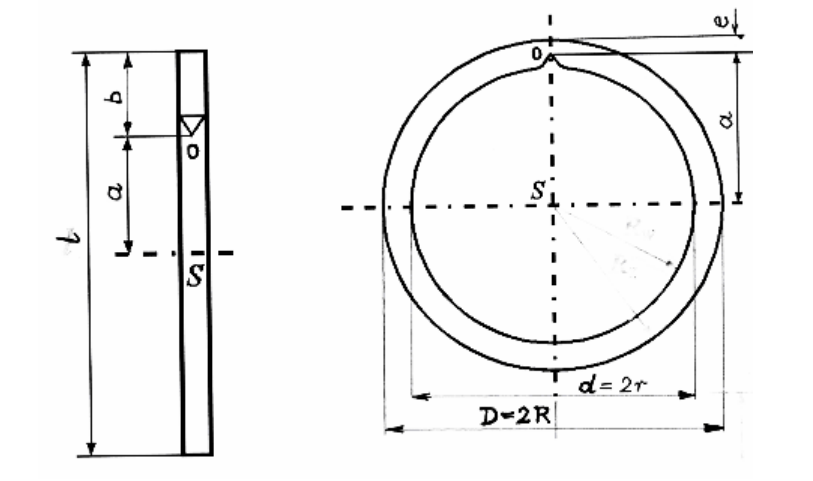
\includegraphics[width=0.8\linewidth]{./schemat}
\caption{Pręt i pierścień używane w ćwiczeniu.}
\end{figure}

\section{Wykonanie ćwiczenia}
Na początku ustalamy masę oraz określamy długości pręta i pierścienia, tak jak pokazano na Rysunku 1 (małe długości mierzymy suwmiarką). Umieszczamy pręt na statywie, wprowadzamy go w ruch drgający o amplitudzie
nieprzekraczającej trzech stopni i mierzymy czas trzydziestu drgań. Pomiar ten powtarzamy dziesięciokrotnie. Analogicznie postępujemy z pierścieniem.

 
\section{Opracowanie wyników pomiarów}

\begin{table}[ht]
\centering
\setlength{\extrarowheight}{2pt}
\caption{\textbf{Pomiar masy i długości pręta.}}
\begin{tabular}{| @{\hspace{8mm}}c @{\hspace{8mm}}| @{\hspace{8mm}}c @{\hspace{8mm}}|@{\hspace{8mm}} c@{\hspace{8mm}}|}
\hline
 & wartość & niepewność  \\ \hline
$m[g]$ & 30 & 37,37 \\ \hline
$l[mm]$ & 30 & 37,22 \\ \hline
$b[mm]$ & 30 & 37,25 \\ \hline
$a[mm]$ & 30 & 37,34 \\ \hline

\end{tabular}
\end{table}

\begin{table}[ht]
\centering
\setlength{\extrarowheight}{2pt}
\caption{\textbf{Pomiar masy i długości pierścienia.}}
\begin{tabular}{| @{\hspace{8mm}}c @{\hspace{8mm}}| @{\hspace{8mm}}c @{\hspace{8mm}}|@{\hspace{8mm}} c@{\hspace{8mm}}|}
\hline
 & wartość & niepewność  \\ \hline
$m[g]$ & 30 & 37,37 \\ \hline
$D_{W}[mm]$ & 30 & 37,22 \\ \hline
$D_{Z}[mm]$ & 30 & 37,25 \\ \hline
$R_{W}[mm]$ & 30 & 37,22 \\ \hline
$R_{Z}[mm]$ & 30 & 37,25 \\ \hline
$e[mm]$ & 30 & 37,34 \\ \hline
$a[mm]$ & 30 & 37,34 \\ \hline

\end{tabular}
\end{table}

\begin{table}[ht]
\centering
\setlength{\extrarowheight}{2pt}
\caption{\textbf{Pomiar okresu drgań dla pręta.}}
\begin{tabular}{|c|c|c|c|}
\hline
Lp. & liczba okresów $k$ & czas $t$ dla $k$ okresów w [$s$] & okres $T_{i}=t/k$ w [$s$] \\ \hline
1 & 30 & 37,37 & 1,245667\\ \hline
2 & 30 & 37,22 & 1,240667\\ \hline
3 & 30 & 37,25 & 1,241667\\ \hline
4 & 30 & 37,34 & 1,244667\\ \hline
5 & 30 & 37,06 & 1,235333\\ \hline
6 & 30 & 37,32 & 1,244000\\ \hline
7 & 30 & 37,31 & 1,243667\\ \hline
8 & 30 & 37,13 & 1,237667\\ \hline
9 & 30 & 37,47 & 1,249000\\ \hline
10 & 30 & 37,38 & 1,246000\\ \hline
\multicolumn{4}{|c|}{Wartość średnia okresu: $\overline{T}= $} \\ \hline
\multicolumn{4}{|c|}{Niepewność: $u(T)$=} \\ \hline
\end{tabular}
\end{table}

\begin{table}[ht]
\centering
\setlength{\extrarowheight}{2pt}
\caption{\textbf{Pomiar okresu drgań dla pierścienia.}}
\begin{tabular}{|c|c|c|c|}
\hline
Lp. & liczba okresów $k$ & czas $t$ dla $k$ okresów w [$s$] & okres $T_{i}=t/k$ w [$s$] \\ \hline
1 & 30 & 37,37 & 1,245667\\ \hline
2 & 30 & 37,22 & 1,240667\\ \hline
3 & 30 & 37,25 & 1,241667\\ \hline
4 & 30 & 37,34 & 1,244667\\ \hline
5 & 30 & 37,06 & 1,235333\\ \hline
6 & 30 & 37,32 & 1,244000\\ \hline
7 & 30 & 37,31 & 1,243667\\ \hline
8 & 30 & 37,13 & 1,237667\\ \hline
9 & 30 & 37,47 & 1,249000\\ \hline
10 & 30 & 37,38 & 1,246000\\ \hline
\multicolumn{4}{|c|}{Wartość średnia okresu: $\overline{T}= $} \\ \hline
\multicolumn{4}{|c|}{Niepewność: $u(T)$=} \\ \hline
\end{tabular}
\end{table}

\subsection{Moment bezwładności $I_{0}$ względem rzeczywistej osi obrotu korzystając z~wzoru na okres drgań}
Wzór na okres drgań wyraża się wzorem:
$$T=2\pi\sqrt{\dfrac{I_{0}}{mga}}$$
Przekształcając odpowiednio powyższe równanie otrzymujemy wzór na moment bezwładności:
$$I_{0}=\dfrac{mgaT^{2}}{4\pi^{2}},$$
gdzie $m$ -- masa bryły, $g$ -- przyspieszenie ziemskie, $T$ -- okres drgań, $a$ -- odległość środka masy od osi obrotu.
$$$$
\textbf{Momement bezdładności $I_{0}$ dla pręta:}
$$I_{0} = $$
\textbf{Momement bezdładności $I_{0}$ dla pierścienia:
}$$I_{0} = $$

\subsection{Moment bezwładności $I_{S}$ względem osi przechodzącej przez środek masy korzystając z twierdzenia Steinera}
Twierdzenie Steinera stosuje się do obliczania momentu bezwładności bryły względem osi przesuniętej równolegle o długość $a$, gdzie $I_{S}$ to moment bezwładności względem osi przechodzącej przez środek masy bryły.
$$I_{0}=I_{S}+ma^{2}$$
$$I_{S}=I_{0}-ma^{2}$$
\textbf{Momement bezdładności $I_{S}$ dla pręta:
}$$I_{S} = $$
\textbf{Momement bezdładności $I_{S}$ dla pierścienia:
}$$I_{S} = $$

\subsection{Moment bezwładności względem osi przechodzącej przez środek masy $I_{S}^{(geom)}$ na podstawie masy i wymiarów geometrycznych}
Moment bezwładności większości regularnych brył można zapisać w postaci: 
$$I_{S}^{(geom)} = k \cdot m \cdot l,$$ 
gdzie $m$ -- masa bryły, $l$ -- charakterystyczny wymiar bryły (np. długość, promień), $k$ -- bezwymiarowy współczynnik
zależny tylko od kształtu bryły i wyboru charakterystycznego wymiaru (np. promień czy średnica), a niezależny od wielkości bryły.
$$$$
\textbf{Momement bezdładności $I_{S}^{(geom)}$ dla pręta:
}$$I_{S}^{(geom)} = \dfrac{1}{12}ml^{2}$$
\textbf{Momement bezdładności $I_{S}^{(geom)}$ dla pierścienia:
}$$I_{S}^{(geom)} = \dfrac{1}{12}m(R^{2}+r^{2})$$

\subsection{Niepewności mierzonych wielkości}
\subsubsection{Niepewność pomiaru okresu -- niepewność typu A}
Wzór na niepewność pomiaru $u(T)$:
$$u(T)=\displaystyle \frac{\sqrt{\frac{\sum(T_{i}-\overline{T})^{2}}{n-1}}}{\sqrt{n}}=\displaystyle \sqrt{\frac{\sum(T_{i}-\overline{T})^{2}}{n(n-1)}},$$
gdzie $n$ -- liczba pomiarów, $\overline{T}=\frac{1}{n}\sum T_{\mathrm{i}}$ -- średni czas trwania okresu.
$$$$
\textbf{Niepewność pomiaru okresu dla pręta:}
$$\overline{T}=$$ 
$$u(T)=\displaystyle \sqrt{\frac{\sum(T_{i}-\overline{T})^{2}}{n(n-1)}}$$
\textbf{Niepewność pomiaru okresu dla pierścienia:}
$$\overline{T}=$$ 
$$u(T)=\displaystyle \sqrt{\frac{\sum(T_{i}-\overline{T})^{2}}{n(n-1)}}$$
\subsubsection{Niepewność pomiaru masy}
Niepewność pomiaru masy jest równa działce elementarnej wagi $u(m)=1g$.
\subsubsection{Niepewność pomiaru wymiarów geometrycznych}
Przyjmujemy niepewność równą działce elementarnej linijki $u(l)=1mm$. Wyjątek stanowi wielkość $e$ wyrażona poprzez różnicę promieni $R_{Z}$ i $R_{W}$, ze względu na małe rozmiary przyjmujemy niepewność pomiaru $u(e)=0,1mm$. Jeśli odległość $a=\dfrac{l}{2}-b$, to analogicznie $u(a)=0,5mm$;
\subsection{Niepewność złożona momentu bezwładności $I_{0}$}
\textbf{Niepewność złożona momentu bezwładności $I_{0}$ dla pręta:}
$$$$
\textbf{Niepewność złożona momentu bezwładności $I_{0}$ dla pierścienia:}

\subsection{Niepewność złożona momentu bezwładności $I_{S}$}
\textbf{Niepewność złożona momentu bezwładności $I_{S}$ dla pręta:}
$$$$
\textbf{Niepewność złożona momentu bezwładności $I_{S}$ dla pierścienia:}

\subsection{Niepewność $u_{c}(I_{S}^{(geom)})$}
\textbf{Niepewność $u_{c}(I_{S}^{(geom)})$ dla pręta:}
$$$$
\textbf{Niepewność $u_{c}(I_{S}^{(geom)})$ dla pierścienia:}

\subsection{Porównanie metod wyznaczenia momentu bezwładności}

\subsection{Zgodność wyników pomiaru w granicach niepewności rozszerzonej}

\begin{table}[ht]
\centering
\caption{\textbf{Wyniki obliczeń momentu bezwładności dla pręta.}}
\begin{tabular}{|c|m{30mm}|m{30mm}|m{30mm}|}
\hline
& $I_{0}$ wyznaczone z~okresu drgań $[kg\cdot m^{2}]$ & $I_{S}$ wyznaczone z~twierdzenia Steinera $[kg\cdot m^{2}]$ & $I_{S}$ wyznaczone z~pomiarów geometrycznych $[kg\cdot m^{2}]$  \\ \hline
wartość & \begin{center}30\end{center} & \begin{center}37,37\end{center} & \begin{center}66\end{center}\\ \hline
niepewność &\begin{center}30\end{center} & \begin{center}37,37\end{center} & \begin{center}66\end{center}\\ \hline

\end{tabular}
\end{table}

\begin{table}[ht]
\centering
\caption{\textbf{Wyniki obliczeń momentu bezwładności dla pierścienia.}}
\begin{tabular}{|c|m{30mm}|m{30mm}|m{30mm}|}
\hline
& $I_{0}$ wyznaczone z~okresu drgań $[kg\cdot m^{2}]$ & $I_{S}$ wyznaczone z~twierdzenia Steinera $[kg\cdot m^{2}]$ & $I_{S}$ wyznaczone z~pomiarów geometrycznych $[kg\cdot m^{2}]$  \\ \hline
wartość & \begin{center}30\end{center} & \begin{center}37,37\end{center} & \begin{center}66\end{center}\\ \hline
niepewność &\begin{center}30\end{center} & \begin{center}37,37\end{center} & \begin{center}66\end{center}\\ \hline

\end{tabular}
\end{table}



\section{Wnioski}
\begin{itemize}
\item 
\item 
\item  
\end{itemize}
\end{document}